\documentclass[a4paper,10pt]{article}
\usepackage[utf8]{inputenc}
\usepackage{amsmath, amssymb, amsthm}
\usepackage{geometry}
\geometry{margin=0.5in}
\usepackage{enumitem}
\usepackage{hyperref}
\usepackage{graphicx}
\newcommand{\R}{\mathbb{R}}

\title{MATH2033 Final Notes}
\begin{document}
\maketitle
\vspace{5cm}
\begin{figure}[ht]
    \centering
    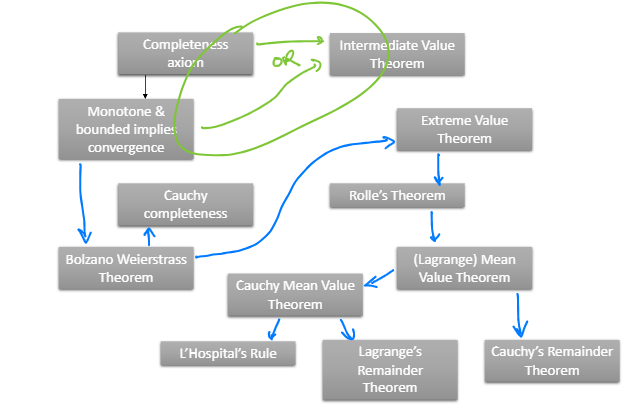
\includegraphics[width=0.8\textwidth]{1023summary.png}
    \caption{The overall logic of MATH1023}
    \label{fig:math2033}
\end{figure}
\newpage


\section{Sets, Sequence, Series}
\subsection{countability}
\begin{center}
    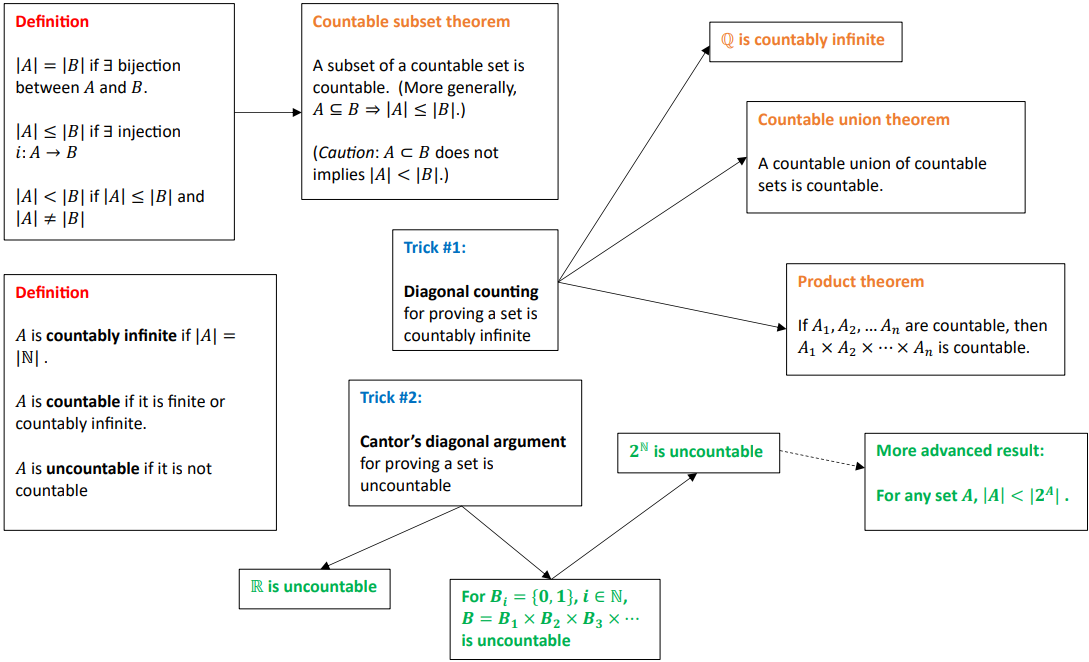
\includegraphics[width=\textwidth]{countability.png} 
\end{center}

\subsection{sup, inf, real numbers}
\noindent Facts that can be directly used:
\begin{itemize}
    \item If $x\leq C \text{ or } x<C$ for all $x\in S$, then $C$ is an upper bound of $S$, and\[
        \sup S \leq C
    \]
    \item $\forall x,y\in A$, we have\[
        |x-y| \leq \sup A - \inf A
    \]
\end{itemize}

\subsection{Limits}
\begin{itemize}
    \item \textbf{Supreme Limit Theorem}: Given a nonempty set $S\subset\R$ with an upper bound $c$, then $c=\sup S$
    iff there exists a sequence $\{x_n\}\subset S$ such that $\lim\limits_{n\to\infty}x_n=c$.
    \item \textbf{Interwining Sequence Theorem}: If $\{a_{2n}\}$ and $\{a_{2n+1}\}$ converge to the same limit $L$, then $\{a_n\}$ converges to $L$.
\end{itemize}

\subsection{series convergence}
\begin{itemize}
    \item \textbf{Summation by parts} Suppose $S_j=\sum_{k=1}^{j}a_k$, then\[
        \sum_{k=1}^{n}a_kb_k = S_n b_n - \sum_{k=1}^{n-1}S_k(b_{k+1}-b_k).
    \]
    \item \textbf{Dirichelet's test}: If $\sum_{k=1}^{\infty}a_k$ is bounded and $\{b_k\}$ is monotone decreasing that converges to $0$, then $\sum_{k=1}^{\infty}a_kb_k$ converges.
    \item \textbf{Generalized Dirichelet's test}: The above test can be generalized to the case where $\{b_k\}$ is not monotone decreasing, but $\sum_{k=1}^{\infty}|b_k-b_{k+1}|$ converges and $b_k\to0$.
    \item \textbf{Cauchy Product Theorem}: If $\sum_{k=0}^{\infty}a_k$ converges \textit{absolutely} and $\sum_{k=0}^{\infty}b_k$ converges, then\[
        \sum_{k=0}^{\infty}a_k b_k = \sum_{k=0}^{\infty}a_k \cdot \sum_{k=0}^{\infty}b_k.
    \]
\end{itemize}

\newpage

\section{$\varepsilon$-type arguments}
It's a good practice to separate terms in $f(x)$ and $|x-x_0|$, either by sum or by product.
\begin{center}
    - Left as sketch paper -
\end{center}

\newpage

\section{Function continuity and differentiability}
\subsection{Function limits}
\noindent The following are some theorems that may be negleted but useful:
\begin{itemize}
    \item \textbf{Sequential Limit Theorem}: For $f:S\to\R$, $\lim\limits_{x\to x_0}f(x)=L$
        iff\[
            \forall \{x_n\} \subset S \setminus \{x_0\} \text{ s.t. } x_n\to x_0 
                        \implies \lim\limits_{n\to\infty}f(x_n)=L.
        \]
        In fact, if $\lim\limits_{n\to\infty}f(x_n)$ exists for every such $x_n\to x_0$, then all the limit values are the same.
        Using this theorem, we can also easily show a function limit do not exist by finding 2 sequences with different limits.
    \item \textbf{Monotone Function Theorem}: If $f$ is increasing on $(a,b)$, then for any $x_0\in(a,b)$, \[
        f(x_0^-) = \sup\{f(x) | a<x<x_0\},
    \]
    and if it is bounded below, then\[
        f(a^+) = \inf\{f(x) | x_0<x<b\}.
    \]
    \textbf{Jump Discontinuity}: moreover, under the condition above, the following set is countable\[
        \{x\in(a,b) | f(x^+)\neq f(x^-)\}.
    \]
\end{itemize}
The following limits can be cited directly:
\begin{itemize}
    \item Let $f(x)=x\sin(\frac{1}{x})$ whenever $x\neq 0$, and $f(0)=0$, then\[
        \lim\limits_{x\to 0}f(x) = \lim\limits_{x\to 0}x\sin(\frac{1}{x}) = 0,
    \]
    which is NOT a result of things like L'Hospital's rule, but a result of the fact that $\sin(\frac{1}{x})$ is bounded plus the Squeeze Theorem.
    \item For any $n\in\mathbb{N}$, let $p_n(x) = a_0 + a_1x + a_2x^2 + \cdots + a_nx^n$, then\[
        \lim\limits_{x\to \infty}p_n(x) = \begin{cases}
            \infty & \text{if } a_n>0\\
            -\infty & \text{if } a_n<0\\
        \end{cases}
    \]
    and \[
        \lim\limits_{x\to 0}\frac{1}{p_n(x)} = 0.
    \]
\end{itemize}

\subsection{Function continuity}
\begin{itemize}
    \item \textbf{Sequential Continuity Theorem}: A function $f$ is continuous at $x_0$ iff\[
        \forall \{x_n\} \subset S \setminus \{x_0\} \text{ s.t. } x_n\to x_0 
                        \implies \lim\limits_{n\to\infty}f(x_n)=f(x_0).
    \]
    \item \textbf{Inverse Function Theorem}: covered at the end of \texttt{lecture 4} and the beginning of \texttt{lecture 5}.
    \item All of the following require to be continuous on $[a,b]$: EVT, Rolle's, MVT, \textbf{Generalized MVT}, which is: $f,g$ continuous on $[a,b]$
    and differentiable on $(a,b)$, then there exists $c\in(a,b)$ such that\[
        g^\prime(c) (f(b)-f(a)) = f^\prime(c)(g(b)-g(a)).
    \]
    \item Relationship between derivative and monotonicity is a little bit complex issue, presented at 
    \textbf{Curve Tracing Theorem} and \textbf{Local Tracing Theorem} in \texttt{lecture 5} Page 6-7.
\end{itemize}
\textbf{Remark:} When finding things like $f(b)-f(a)$ with $f'(x)$ consider use the MVT or GMVT for proving equations or inequalities.

\newpage

\section{Taylor Approximation, Lagrange Remainder, Taylor Series}
\subsection{Taylor's Theorem}
Let $f:(a,b)\to\R$ be $n$ times differentiable on $(a,b)$. For every $x,c\in(a,b)$, there exists $x_0$
between $x$ and $c$ such that\[
    f(x) = f(c) + f^\prime(c)(x-c) + \frac{f^{\prime\prime}(c)}{2!}(x-c)^2 + \cdots + \frac{f^{(n)}(c)}{n!}(x-c)^n + R_n(x),
\]
where $R_n(x)$ is the Lagrange remainder:
\[
    R_n(x) = \frac{f^{(n+1)}(x_0)}{(n+1)!}(x-c)^{n+1}.
\]
As a corralary, if $f\in C^\infty$, and for $x\in(a,b)$, if $\lim\limits_{n\to\infty}R_n(x)=0$, then\[
    f(x) = \sum_{k=0}^\infty \frac{f^{(k)}(c)}{k!}(x-c)^k,
\]
which is called the Taylor series of $f$ at $c$.\\
\textbf{Remark:} This is the result of MVT and is a property on an interval.

\subsection{Taylor Polynomial}
Given that $f$ is $n$-times differentiable at $x = a$, then
\[
    f(x) = \sum_{k=0}^n \frac{f^{(k)}(a)}{k!}(x - a)^k + o((x-a)^n)
\]
as $x \to a$.
The polynomial
\(
    P_n(x) = \sum_{k=0}^n \frac{f^{(k)}(a)}{k!}(x - a)^k
\)
which we will denote by $T_a^n(x)$ or simply $T_n(x)$ in this course, is called the $n$-th degree Taylor polynomial (or approximation) of $f$ near $x = a$.
This can be used to approximate $f(x)$ for $x$ near $a$, and will be useful in n-th derivative tests.

\noindent A function $f$ is said to be real analytic at $x = a$ if there exists a neighborhood of $a$ such that
\[
    f(x) = \sum_{k=0}^\infty \frac{f^{(k)}(a)}{k!}(x - a)^k
\]
for all $x$ in that neighborhood.\\
\textbf{Remark:} This is the result of L'Hospital's rule and is a property at a point.

\subsection{Techniques}
\begin{itemize}
    \item \textbf{Remark 1:} When dealing with $m$-times differentiable functions and terms like $f, f', f''$ with coefficients such as $\frac{1}{2}, \frac{1}{6}$, consider using Taylor's theorem.
    \item When finding $\sup$ or $\inf$, use the facts:
    \begin{align*}
        \forall x\in S,\, x \leq M &\implies \sup S \leq M\\
        \exists x\in S,\, x \leq M &\implies \inf S \leq M
    \end{align*}
    where $M$ can be any value.
    \item \textbf{Remark 2:} For expressions like $(f(x) + f'(x))$ with information about $f$, consider constructing a helper function $F(x)$ as a combination of $f(x)$ and $e^x$.
    \item \textbf{Remark 3:} When applying L'Hospital's rule, remember it cannot be used to prove divergence. For example:
    \[
        \lim_{x\to 0}\frac{x^2\sin\frac{1}{x}}{\sin x}, \qquad \lim_{x\to\infty}\frac{x + \sin x}{x}
    \]
\end{itemize}



\newpage

\section{Integration}
\subsection{integral criterion}
If $f$ is bounded on $[a,b]$, $f$ is integrable if and only if,
given any $\varepsilon>0$, there exists a partition $P$ of $[a,b]$ such that\[
    U(f,P) - L(f,P) < \varepsilon,
\]
where \[
    U(f,P) = \sum_{i=1}^n M_i\Delta x_i, \quad L(f,P) = \sum_{i=1}^n m_i\Delta x_i,
\]
and $M_i$ and $m_i$ are the supremum and infimum of $f$ on the interval $[x_{i-1}, x_i]$, respectively.\\

\noindent For a bounded function $f$ on $[a,b]$, $f$ is integrable on $[a,b]$ iff $f$ is continuous everywhere except 
on a set of measure zero, i.e. the set\[
    \{x\in[a,b] | S_f \text{ is discontinuous at } x\}
\]
is a set of measure zero (make sure it's continuous on other points), i.e. for any $\varepsilon>0$,
there exists countable number of intervals $(a_i,b_i)$ such that\[
    \sum_{i=1}^\infty (b_i-a_i) < \varepsilon, \text{   and   } S_f\subseteq \bigcup_{i=1}^\infty (a_i,b_i) 
\]
Note: A countable union of sets of measure zero is a set of measure zero.\\

\noindent Given this, we may find the following to be integrable:\begin{itemize}
    \item By Monotone Function Theorem, if $f$ is monotone on $[a,b]$, then $f$ is integrable on $[a,b]$.
    \item If $f$ is continuous except a convergent sequence of points $x_n\to c$ in $[a,b]$, then $f$ is integrable on $[a,b]$.
    This follows directly from choosing proper $\delta$, DO NOT use the tidious function value when encontering
    some realization of such $f$.
\end{itemize}
\subsection{integral rules}
\begin{itemize}
    \item \textbf{FTC:}\begin{itemize}
        \item If $f$ is integrable on $[a,b]$, continuous at $x_0\in[a,b]$ and $F(x)=\int_a^x f(t)dt$, then $F$ is continuous on $[a,b]$ and differentiable at $x_0$, and\(
            F'(x_0) = f(x_0).
        \)
        \item If $G$ is differentiable on $[a,b]$ and $G'(x)=g(x)$ for all $x\in[a,b]$, then\(
            \int_a^b g(x)dx = G(b) - G(a).
        \)\end{itemize}
    \item \textbf{By parts:} If $f,g$ are continuous on $[a,b]$, then\(
        \int_a^b f(x)g'(x)dx = f(b)g(b) - f(a)g(a) - \int_a^b g(x)f'(x)dx.
    \)
    \item \textbf{Substitution:} If $f$ is continuous on $[a,b]$, and $g$ is differentiable on $[c,d]$ then \(
        \int_a^b f(g(x))g'(x)dx = \int_{g(a)}^{g(b)} f(u)du
    \)
    
\end{itemize}
\subsection{integral test}
\begin{itemize}
    \item \textbf{p-test}
    \begin{align*}
        \int_1^\infty \frac{1}{x^p} dx &\text{ converges iff } p>1\\
        \int_0^1 \frac{1}{x^p} dx &\text{ converges iff } p<1\\
    \end{align*}
    \item \textbf{Comparison Test}
    \item \textbf{Limit Comparison Test}: Suppose $f,g$ are positive functions on $\R$, define $L:=\lim\limits_{x\to\infty}\frac{f(x)}{g(x)}$, then\begin{itemize}
        \item If $0<L<\infty$, then $\int_1^\infty f(x)dx$ converges iff $\int_1^\infty g(x)dx$ converges.
        \item If $L=0\;$, $\int_1^\infty f(x)dx$ converges $\implies$ $\int_1^\infty g(x)dx$ converges.
        \item If $L=\infty$, $\int_1^\infty g(x)dx$ converges $\implies$ $\int_1^\infty f(x)dx$ converges.
    \end{itemize}
    \item \textbf{Absolute Convergence Test}
\end{itemize}
\textbf{Remark:} When nothing works, consider the function\[
    F(x) = \int_1^x f(t)dt
\]
and calculate the limit directly. Theoretically, this will always give a result.




\newpage
\appendix
\section{Appendix}
\subsection{Limits that can be used directly}
\begin{align*}
    \lim\limits_{x\to 0}\frac{\sin x}{x} &= 1,\\
    \lim\limits_{x\to 0}\frac{x^r}{e^x} &= 0 \text{ for any } r\in\R,\\
    \lim\limits_{n\to\infty} \left(1 + \frac{1}{n}\right)^n &= e,\\
    \lim\limits_{x\to 0} (1 + x)^{1/x} &= e,\\
\end{align*}

\subsection{Triangular Equations}
\begin{align*}
    \sin^2\theta + \cos^2\theta &= 1 \\
    1 + \tan^2\theta &= \sec^2\theta \\
    1 + \cot^2\theta &= \csc^2\theta \\
    \tan\theta &= \frac{\sin\theta}{\cos\theta} \\
    \sin(\theta \pm \varphi) &= \sin\theta\cos\varphi \pm \cos\theta\sin\varphi \\
    \cos(\theta \pm \varphi) &= \cos\theta\cos\varphi \mp \sin\theta\sin\varphi \\
    \tan(\theta \pm \varphi) &= \frac{\tan\theta \pm \tan\varphi}{1 \mp \tan\theta\tan\varphi} \\
    \sin(2\theta) &= 2\sin\theta\cos\theta \\
    \cos(2\theta) &= \cos^2\theta - \sin^2\theta \\
                  &= 1 - 2\sin^2\theta \\
                  &= 2\cos^2\theta - 1 \\
    \tan(2\theta) &= \frac{2\tan\theta}{1 - \tan^2\theta} \\
    \sin^2\theta &= \frac{1 - \cos(2\theta)}{2} \\
    \cos^2\theta &= \frac{1 + \cos(2\theta)}{2} \\
    2\sin\theta\cos\varphi &= \sin(\theta + \varphi) + \sin(\theta - \varphi) \\
    2\cos\theta\cos\varphi &= \cos(\theta + \varphi) + \cos(\theta - \varphi) \\
    2\sin\theta\sin\varphi &= \cos(\theta - \varphi) - \cos(\theta + \varphi) \\
    \sin\theta + \sin\varphi &= 2\sin\left(\frac{\theta + \varphi}{2}\right)\cos\left(\frac{\theta - \varphi}{2}\right) \\
    \sin\theta - \sin\varphi &= 2\cos\left(\frac{\theta + \varphi}{2}\right)\sin\left(\frac{\theta - \varphi}{2}\right) \\
    \cos\theta + \cos\varphi &= 2\cos\left(\frac{\theta + \varphi}{2}\right)\cos\left(\frac{\theta - \varphi}{2}\right) \\
    \cos\theta - \cos\varphi &= -2\sin\left(\frac{\theta + \varphi}{2}\right)\sin\left(\frac{\theta - \varphi}{2}\right) \\
    \sin m \sin \frac{1}{2} &= \frac{1}{2}(\cos(m - \frac{1}{2}) - \cos(m + \frac{1}{2})) \\
    \sin (n\theta) \sin \frac{\theta}{2} &= \frac{1}{2}(\cos((n - \frac{1}{2})\theta) - \cos((n + \frac{1}{2})\theta)) \\
\end{align*}
\end{document}